\chapter{Synthetic Proof of Function}

\section{Purpose and claim boundary}

The experiment verifies that the proposed pipeline is executable, that withheld novelty can be evaluated, that relational reuse contributes a separate signal, and that inclusion monitoring can identify planted process burdens. It is intentionally small and transparent. It does not simulate a country's population, a vendor matcher, human behaviour, or real fraud economics.

\claimboundary

\section{Generator}

The controlled generator creates 12,000 events across 24 synthetic months, 6,500 identities, 1,800 devices, 45 issuers, four channels, and five credential types. Each event contains score-level face and fingerprint evidence, optional iris, quality, liveness, document score, issuer trust, credential status, device risk, velocity, process attempts, duration, and labels known only to the experiment.

Fraud is planted in two families:

\begin{enumerate}
\item \textbf{Known patterns} with degraded matcher/document/liveness evidence, risky devices, and high velocity. These examples are available to supervised training.
\item \textbf{Novel coherence patterns} with plausible fingerprint, liveness, and document scores but an unusual cross-modal combination, including low face compatibility. These examples are excluded from supervised training labels and are intended to test anomaly and graph contribution.
\end{enumerate}

Fraud events reuse a limited device pool to produce relational signal. Legitimate exclusion cases receive additional attempts, longer duration, and quality burden, particularly in a planted kiosk and late partner-channel regime. These process cases must never increase fraud risk merely because the citizen struggled.

\section{Temporal split and leakage controls}

The final 25\% of the time horizon is held out. Preprocessing and models are fit on the earlier period. Novel fraud is withheld from the supervised label set. Device-reuse counts are computed from training evidence only. No target label is used as an input feature.

This split is still weaker than a full industrial evaluation. A future protocol will separate complete rings, issuers, sites, projects, credential campaigns, and model versions, and will include a composition holdout combining known factors in unseen ways.

\section{Models}

The demonstration uses:

\begin{itemize}
\item a class-weighted random forest for known-fraud patterns;
\item Isolation Forest trained on nominal evidence;
\item a device-reuse and device-risk relational baseline;
\item robust channel-conditioned duration and attempt scoring for exclusion;
\item fixed weighted fusion $w_S=0.50$, $w_A=0.25$, $w_G=0.25$.
\end{itemize}

The relational component is deliberately not called a GNN. It is a baseline that tests the graph hypothesis before model complexity. The separate GNN repository remains the appropriate experimental line for full message passing and ring-held-out comparisons.

\section{Results}

The temporal test set contains \TestN{} events at a fraud prevalence of \FraudRate{}. The hybrid score obtains ROC AUC \RocAuc{}, average precision \AvgPrecision{}, and Brier score \Brier{}. At a top-\ReviewCapacity{} review capacity, fraud recall is \RecallCapacity{} and recall on deliberately withheld novel fraud is \NovelRecall{}. The process-exclusion score obtains ROC AUC \ExclusionAuc{} against planted exclusion labels.

\begin{figure}[htbp]
\centering
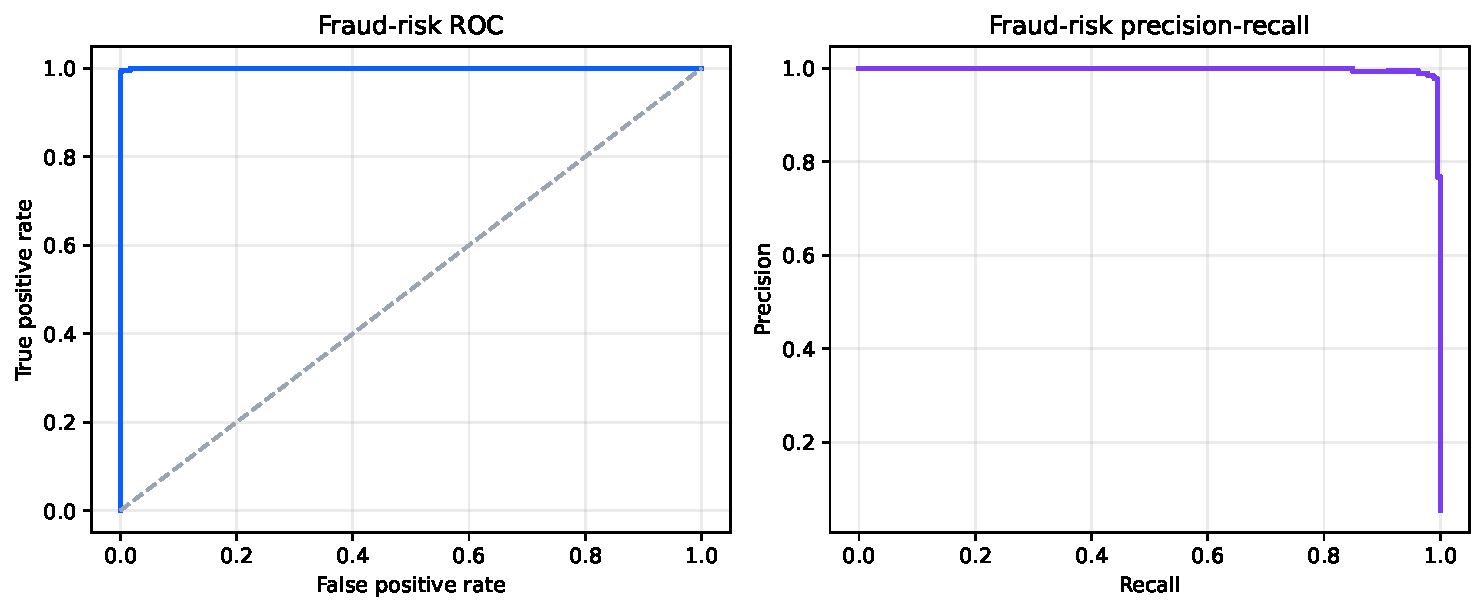
\includegraphics[width=0.92\textwidth]{../figures/fraud_curves.pdf}
\caption{Synthetic fraud-ranking curves. These are pipeline checks, not operational product claims.}
\label{fig:fraud-curves}
\end{figure}

\begin{figure}[htbp]
\centering
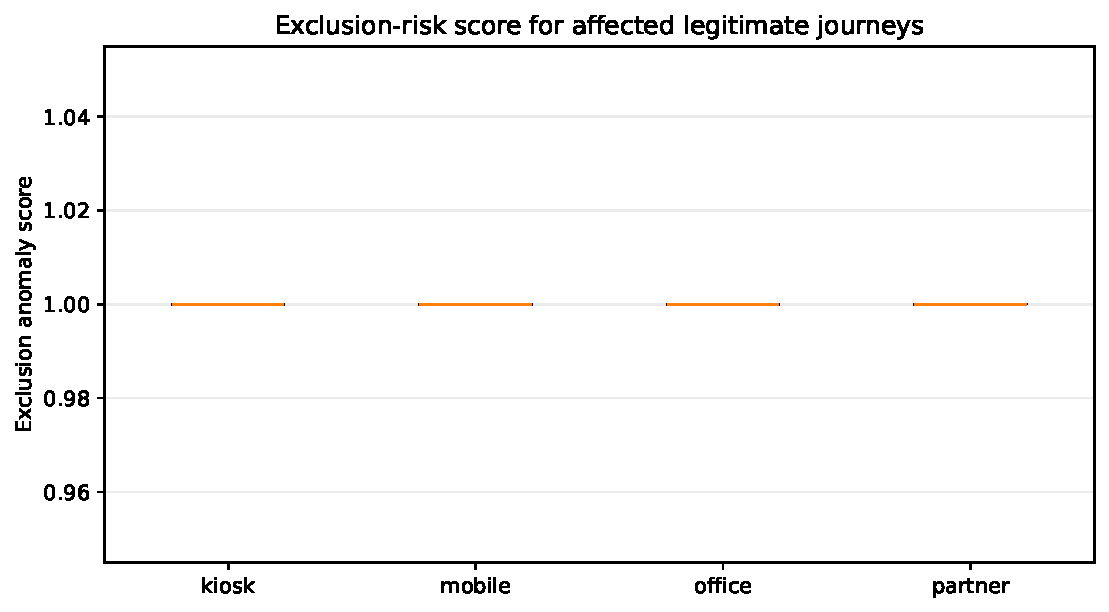
\includegraphics[width=0.78\textwidth]{../figures/exclusion_by_channel.pdf}
\caption{Synthetic exclusion scores for planted affected legitimate journeys by channel.}
\label{fig:exclusion}
\end{figure}

The expected interpretation is limited. High performance is partly a property of the planted generator. It confirms that the code, split, score fusion, metrics, and paper-generation chain are coherent. It does not validate feature realism, attacker adaptation, fairness, calibration transfer, legal admissibility, or field utility.

\section{Required ablations}

A publishable empirical programme must compare:

\begin{enumerate}
\item rules only;
\item logistic regression and tree baselines;
\item supervised model only;
\item anomaly model only;
\item relational structural baseline;
\item GNN with ring-held-out split;
\item supervised + anomaly;
\item supervised + graph;
\item full hybrid;
\item full hybrid with action policy and inclusion observatory.
\end{enumerate}

Additional ablations remove modality quality, component provenance, graph edge types, regime conditioning, remedy features, and synthetic hard negatives. A permuted graph and permuted regime assignment test whether improvements depend on meaningful structure.

\section{Field-validation protocol}

Field validation proceeds in five gates:

\begin{description}
\item[Gate 0 --- Contract.] Agree purpose, outcomes, ground-truth states, evidence, retention, actions, review, and remedy.
\item[Gate 1 --- Retrospective.] Replay historical events without changing decisions; measure leakage, calibration, segments, and label quality.
\item[Gate 2 --- Shadow.] Run prospectively with no user or operator impact; compare current and proposed decisions.
\item[Gate 3 --- Controlled support.] Rank a bounded expert queue and recommend evidence gaps; the authorized process retains final control.
\item[Gate 4 --- Governed production.] Automate only approved low-risk actions, with rollback, monitoring, appeal, and independent assurance.
\end{description}

The study must pre-register primary metrics and stopping conditions. A system may be technically predictive and still receive REDESIGN or NO-GO because purpose, proportionality, inclusion, explainability, or remedy is inadequate.

\section{Threats to validity}

\begin{itemize}
\item \textbf{Synthetic realism}: planted patterns may be easier than real fraud.
\item \textbf{Selection bias}: confirmed fraud overrepresents cases that current systems can already detect.
\item \textbf{Investigation bias}: review capacity shapes the labels used for training.
\item \textbf{Temporal adaptation}: attackers respond to deployed controls.
\item \textbf{Context shift}: sites, devices, issuers, and policies change.
\item \textbf{Graph error}: shared infrastructure can be legitimate and edges may be stale.
\item \textbf{Outcome ambiguity}: anomaly, administrative error, attempted fraud, and confirmed fraud require separate states.
\item \textbf{Fairness measurement}: aggregate parity can hide individual and intersectional harm.
\item \textbf{Automation bias}: human review can amplify rather than correct a model signal.
\end{itemize}

